%% is_hypergamy_real: short fun paper, first version 2026-10-28; "Beyond status" update 2026-10-28;
%% Dark Triad, paternity and red-flags update 2026-10-28; re-check update (bad boys split, 17:1, N1c, France) 2026-10-28.
%% Sources: ../literature_review.md, ../notes.md, ../bibliography.bib (verified keys only).
%% Every number in the text comes from ../notes.md; see paper/notes.md for the list.
\documentclass[conference,a4paper]{IEEEtran}
\usepackage[T1]{fontenc}
\usepackage[utf8]{inputenc}
\usepackage[table]{xcolor}
\usepackage{microtype,booktabs,amsmath,amssymb,array}
\usepackage{tikz}
\usetikzlibrary{arrows.meta,positioning,calc,patterns,shapes.multipart,shapes.geometric,shadows,decorations.pathreplacing}
\usepackage{pgfplots}
\pgfplotsset{compat=1.18}
\usepgfplotslibrary{groupplots,fillbetween}

% Figure palette (Okabe--Ito, colour-blind safe), defined once and used by every figure.
% In greyscale: hgblue reads dark, hgverm and hggreen mid, hgorange and hgsky light;
% figures add a pattern, line style or marker wherever two colours must be told apart.
\definecolor{hgblue}{HTML}{0072B2}
\definecolor{hgverm}{HTML}{D55E00}
\definecolor{hgorange}{HTML}{E69F00}
\definecolor{hggreen}{HTML}{009E73}
\definecolor{hgsky}{HTML}{56B4E9}
\definecolor{hgink}{HTML}{2B2B2B}
\tikzset{
  hgshadow/.style={drop shadow={opacity=0.22, shadow xshift=0.7pt, shadow yshift=-0.7pt}},
  hgbadge/.style={draw=hgink, fill=white, rounded corners=1.5pt, font=\scriptsize, align=center, inner sep=2pt},
}
\usepackage{eurosym}
\usepackage{cite}
\usepackage[hidelinks]{hyperref}

% Verdict symbols for Table I (black and grey only).
\DeclareRobustCommand{\vexists}{\tikz[baseline=-0.6ex]\fill[black] (0,0) circle (2.6pt);}
\DeclareRobustCommand{\vpartly}{\tikz[baseline=-0.6ex]{\draw[black] (0,0) circle (2.6pt);\fill[black] (0,0) -- (90:2.6pt) arc (90:270:2.6pt) -- cycle;}}
\DeclareRobustCommand{\vnot}{\tikz[baseline=-0.6ex]\draw[black, thick] (0,0) circle (2.4pt);}
\DeclareRobustCommand{\vunclear}{\tikz[baseline=-0.6ex]{\fill[black!30] (0,0) circle (2.6pt);\node[font=\tiny\bfseries, inner sep=0] at (0,0) {?};}}

\title{Marrying Up, Messaging Up, Making It Up:\\ Where Hypergamy Is Real, Half Real and Not Real}

\author{\IEEEauthorblockN{Umay~\c{S}aml\i{}}
\IEEEauthorblockA{\textit{Independent researcher}\\
samliumay965@gmail.com}}

\begin{document}
\bstctlcite{IEEEexample:BSTcontrol}
\maketitle

\begin{abstract}
Online, ``hypergamy'' is used as a law of nature: women always marry up, and most of them chase the top 20\% of men. In the research literature the word covers at least four separate claims, and the evidence differs for each. We sort published findings by claim. On average, women in almost every country studied say a partner's earning prospects matter more to them than men say, but the gap is small on any single trait, and both sexes rank kindness and intelligence higher. Once people meet face to face, earning prospects predict attraction only weakly, and about equally for both sexes. Women marrying up in education was the norm for most of the twentieth century and has now reversed in most countries, which models explain by supply alone. Women still tend to partner with men who earn more and who are a few years older. The ``80/20'' claim is not supported: attention on dating sites is unequal, but men and women aim above themselves by about the same amount, and most couples match like with like. Beyond status, women's stronger interest in status is mostly a long-term preference, and ovulation shifts have not held up. Height, build, penis size and intelligence count in ratings, mostly by small amounts. Most famous dating-app numbers, such as the ``Gini of likes'', come from blogs. On ``bad boys'' the evidence splits: people high in narcissism and psychopathy report more partners, and narcissists of both sexes are chosen more at first meetings, mostly through looks and boldness. No study finds dark traits preferred for the long term. The claim that 10 to 30\% of children are not their presumed father's fails: population rates are about 1 to 2\%. Fewer men than women did pass on their genes: the female effective population size was about twice the male over the long run and up to 17 times larger 8,000 to 4,000 years ago. The cause is debated. Racial hierarchies on dating sites are well documented, and we treat them as discrimination. We close with the Hypergamy Meter, a desktop toy whose hand-picked weights make it a joke, not a measurement. It leaves ethnicity out on purpose.
\end{abstract}

\begin{IEEEkeywords}
hypergamy, assortative mating, mate preferences, online dating, educational hypogamy, Dark Triad, paternity, satire
\end{IEEEkeywords}

\section{Introduction}
Ask the internet whether hypergamy is real and you will be told, with great confidence, that it is the master key to modern dating. In this version, women only ever partner with men above them, status is all that matters, and a small elite of men gets most of the attention while everyone else is left out.

Sociology and psychology use the word more narrowly. Hypergamy usually means a pattern in couples: the woman's partner ranks above her on some dimension, such as education \cite{esteve2012,esteve2016}. Mate-preference research asks a separate question, namely what people \emph{say} they want \cite{buss1989,walter2020}, and dating research asks a third: whom people actually contact, like and marry \cite{eastwick2014,bruch2018,hitsch2010aer}. Online arguments slide between these, so evidence for one claim gets passed off as proof of another.

This paper sorts the claims and checks each one against the evidence. It is a side project and it has a joke app attached (Section~\ref{sec:app}), but the review is meant to be accurate. Our contributions are:
\begin{itemize}
\item a split of ``hypergamy'' into four claims, each with the kind of data that could support it (Fig.~\ref{fig:concept});
\item a verdict for each claim, graded by strength of evidence (Table~\ref{tab:verdict});
\item a short account of the three main explanations, including a supply-based model in which hypergamy appears and then reverses without anyone's preferences changing \cite{grow2015};
\item two more verdict tables, for claims beyond status and for personality and paternity (Tables~\ref{tab:beyond} and~\ref{tab:darkpat}), and an evidence grade for each famous dating-app number (Table~\ref{tab:appnums});
\item a description of the Hypergamy Meter, and a plain statement of why its output means nothing.
\end{itemize}

\section{Four Meanings of ``Hypergamy''}
\label{sec:defs}
Fig.~\ref{fig:concept} shows the four meanings we use throughout.

\textbf{D1, partnering up.} In a couple, the man ranks above the woman on education, income, occupation, class or age. The evidence is the share of couples in which he is higher, compared with what random pairing would give, and it comes from censuses, registers and couple surveys.

\textbf{D2, stated preference.} Women say they weigh a partner's status or earnings more than men do. The evidence is questionnaire ratings.

\textbf{D3, revealed preference and actual matching.} Whom people contact, reply to, swipe on, date and marry. The evidence is dating-site logs, speed dating, field experiments and marriage records.

\textbf{D4, the strong online claim.} Most women pursue a small top fraction of men (``80/20''), and status is all that matters. The evidence would have to show that both attention and actual partnering are concentrated on a few men.

None of these implies another. D1 can appear even when nobody prefers it, because of who is available (Section~\ref{sec:explain}), and a stated preference (D2) may say little about whom people end up liking (D3) \cite{eastwick2008,eastwick2014}. Attention on an app (D3, first contact) is not the same thing as who ends up in a couple (D4 is about both).

\begin{figure}[t]
\centering
% Fig. 1: the four meanings of "hypergamy" (concept map). Pure TikZ, black/grey.
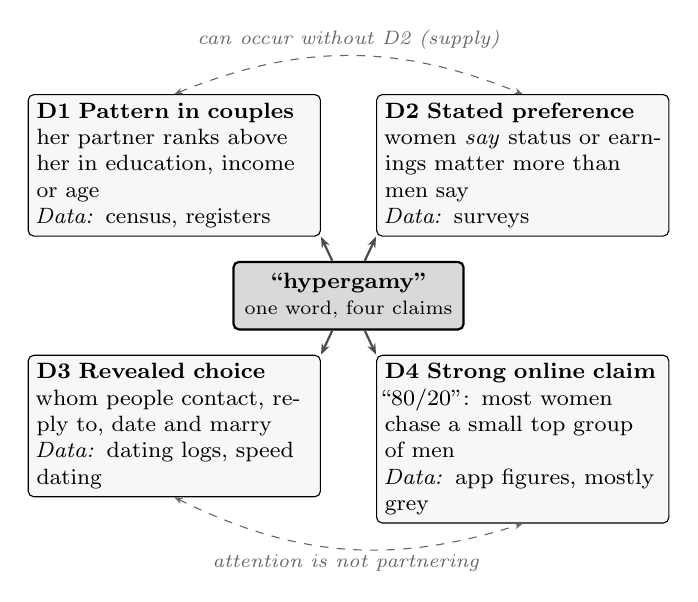
\begin{tikzpicture}[
  font=\footnotesize,
  hub/.style={draw, thick, rounded corners=2pt, fill=black!15, align=center, inner sep=4pt},
  mean/.style={draw, rounded corners=2pt, align=left, text width=3.5cm, inner sep=3pt, fill=black!3},
  link/.style={-{Stealth[length=4pt]}, black!70, thick},
  gap/.style={dashed, black!60, {Stealth[length=3pt]}-{Stealth[length=3pt]}},
  lab/.style={font=\scriptsize\itshape, fill=white, inner sep=1pt, align=center},
]
\node[hub] (h) at (0,0) {\textbf{``hypergamy''}\\{\scriptsize one word, four claims}};
\node[mean, anchor=south east] (d1) at (-0.35, 0.75)
  {\textbf{D1 Pattern in couples}\\ her partner ranks above her in education, income or age\\
   \textit{Data:} census, registers};
\node[mean, anchor=south west] (d2) at (0.35, 0.75)
  {\textbf{D2 Stated preference}\\ women \emph{say} status or earnings matter more than men say\\
   \textit{Data:} surveys};
\node[mean, anchor=north east] (d3) at (-0.35,-0.75)
  {\textbf{D3 Revealed choice}\\ whom people contact, reply to, date and marry\\
   \textit{Data:} dating logs, speed dating};
\node[mean, anchor=north west] (d4) at (0.35,-0.75)
  {\textbf{D4 Strong online claim}\\ ``80/20'': most women chase a small top group of men\\
   \textit{Data:} app figures, mostly grey};
\foreach \d in {d1.south east,d2.south west,d3.north east,d4.north west} \draw[link] (h) -- (\d);
\draw[gap] (d1.north) to[bend left=22] node[lab, above=1pt] {can occur without D2 (supply)} (d2.north);
\draw[gap] (d3.south) to[bend right=22] node[lab, below=1pt] {attention is not partnering} (d4.south);
\end{tikzpicture}

\caption{The four meanings of ``hypergamy'' used in this paper. Evidence for one is not evidence for another: D1 can arise from supply alone, D2 predicts D3 weakly once people meet, and attention on an app (D3, D4) is not partnering.}
\label{fig:concept}
\end{figure}

\section{Evidence by Claim}
\label{sec:evidence}
Table~\ref{tab:verdict} summarises the verdicts. \emph{Strong} means several large or representative studies or meta-analyses agree; \emph{moderate} means good studies with some disagreement or limited settings; \emph{weak} means small, local, grey or unreplicated work.

\begin{table*}[t]
\centering
\caption{Verdict table: \vexists{} exists, \vpartly{} partly, \vnot{} does not exist (as stated), \vunclear{} unclear.}
\label{tab:verdict}
\scriptsize
\renewcommand{\arraystretch}{1.1}
\setlength{\tabcolsep}{4pt}
\begin{tabular}{@{}>{\raggedright\arraybackslash}p{5.85cm} c c >{\raggedright\arraybackslash}p{4.5cm} l >{\raggedright\arraybackslash}p{2.9cm}@{}}
\toprule
\textbf{Claim} & \textbf{Def.} & & \textbf{Verdict} & \textbf{Strength} & \textbf{Main sources}\\
\midrule
\rowcolor{black!6}
Women, on average, \emph{say} earning prospects matter more than men say & D2 & \vexists & exists, in nearly every country studied & strong & \cite{buss1989,walter2020,conroybeam2015,zhang2019}\\
That stated difference is large & D2 & \vpartly & small per trait, large only when many traits are combined & strong & \cite{walter2020,conroybeam2015}\\
\rowcolor{black!6}
Both sexes rank kindness and intelligence above money and looks & D2 & \vexists & exists & strong & \cite{buss1989,walter2020}\\
The stated sex difference shrinks with gender equality & D2 & \vunclear & some studies yes; largest replications no, except for age gaps & moderate & \cite{zentner2012,kasser1999,zhang2019,walter2020}\\
\rowcolor{black!6}
Stated status preferences predict in-person attraction, more for women & D2$\to$D3 & \vnot & mostly not: weak for both sexes, no reliable sex difference & strong (contested) & \cite{eastwick2008,eastwick2014}\\
When screening profiles online, women weight a man's education or income more & D3 & \vexists & exists & moderate & \cite{hitsch2010qme,neyt2019,skopek2011}\\
\rowcolor{black!6}
Women marry up in education & D1 & \vpartly & historically yes; now reversed in most countries & strong & \cite{esteve2012,esteve2016,vanbavel2018,qian2017}\\
Educational hypergamy reflected a wish to marry up & D1 & \vnot & not needed: supply plus a taste for similarity reproduces it & moderate (model) & \cite{grow2015,dehauw2017}\\
\rowcolor{black!6}
Women partner with men who earn more & D1 & \vexists & exists, and persists after the education reversal & strong & \cite{qian2017,chudnovskaya2020}\\
That income gap shows women's preference for higher earners & D1 & \vpartly & mixed with pay gap, selection and men's choices & moderate & \cite{chudnovskaya2020,fisman2006,autor2019}\\
\rowcolor{black!6}
A breadwinner norm shows as a drop where wives start to out-earn husbands & D1 & \vunclear & the drop exists; its reading is contested & moderate & \cite{bertrand2015,binder2022,zinovyeva2021,rosenberg2024}\\
Women partner with older men & D1 & \vexists & about 2 to 3 years on average & strong & \cite{kenrick1992,walter2020,antfolk2017}\\
\rowcolor{black!6}
Marriages where she ``married down'' are less stable & D1 & \vnot & not in recent US cohorts & moderate & \cite{schwartz2014,vanbavel2018}\\
Women trade beauty for men's status & D1 & \vunclear & much apparent exchange is like-with-like matching & moderate & \cite{mcclintock2014,gullickson2017,mcclintock2017}\\
\rowcolor{black!6}
Aiming above oneself is a female trait & D3 & \vnot & both sexes aim up by similar amounts & strong & \cite{bruch2018,kreager2014}\\
Attention on dating apps is unequal; men get fewer replies & D3 & \vexists & exists & moderate & \cite{bruch2018,kreager2014,tyson2016}\\
\rowcolor{black!6}
Most women chase the top $\sim$20\% of men, leaving most men out & D4 & \vnot & not supported as stated & moderate & \cite{bruch2018,kreager2014,rudder2009}\\
Some groups of women face fewer ``marriageable'' men & D1 & \vexists & exists for some groups and places & moderate to strong & \cite{lichter2020,autor2019,raymo2005}\\
\rowcolor{black!6}
Same-sex couples show the same status patterns & D1 & \vunclear & thin evidence; less homogamy overall & weak to moderate & \cite{bailey1994,lippa2007,schwartz2009samesex}\\
\bottomrule
\end{tabular}
\end{table*}

\subsection{Stated Preferences (D2)}
Buss surveyed 37 samples in 33 countries ($N=10{,}047$) \cite{buss1989}. In most samples women rated ``good financial prospects'' and ambition higher than men did, and men rated youth and looks higher. A pre-planned replication in 45 countries ($N=14{,}399$) found the same direction \cite{walter2020}. On a 1 to 7 scale, women rated financial prospects about 0.30 points higher than men, and men rated physical attractiveness about 0.27 points higher. Both sexes rated kindness, intelligence and health above money and looks.

Whether that is a big difference depends on how you count. Per trait, it is small. Across all 18 items of the 1989 data the multivariate distance is $D=2.41$, about 22.8\% overlap, and sex can be predicted from a person's preference profile with 92.2\% accuracy \cite{conroybeam2015}. Across five items in the 2020 data it is $D=0.73$ \cite{walter2020}. Multivariate distances grow with the number of items, so an honest report gives both: single traits overlap heavily, while whole profiles differ more.

Does the gap shrink where women have more equality? Some studies say yes \cite{kasser1999,zentner2012}, as social role theory predicts \cite{eagly1999,wood2002}. The largest and most careful replications found little moderation except for age gaps \cite{zhang2019,walter2020}, and neighbouring countries are not independent data points \cite{gangestad2006}. The difference appears in every country studied. Whether equality shrinks it is still open.

\subsection{Stated Versus Revealed Preferences (D2 to D3)}
In speed dating, the stated sex difference in caring about earning prospects did not predict whom people liked after meeting \cite{eastwick2008}. A meta-analysis of 97 studies reports that attractiveness predicts romantic evaluations at about $r=.40$ and earning prospects at about $r=.10$ for \emph{both} sexes, with a sex difference near .03 \cite{eastwick2014} (Fig.~\ref{fig:stated}). Critics say this covers early attraction and existing couples rather than long-term choice from a wide pool, so the debate continues.

\begin{figure}[t]
\centering
% Fig.: stated versus revealed preferences. DATA, two sources, nothing estimated here.
% (a) walter2020: women rated financial prospects about 0.30 points higher than men,
%     men rated physical attractiveness about 0.27 points higher (1 to 7 scale).
% (b) eastwick2014 (meta-analysis, 97 studies, read from an author copy): after meeting,
%     attractiveness predicts romantic evaluations at about r = .40 and earning prospects
%     at about r = .10, for both sexes; sex difference about .03.
% Greyscale: attractiveness = solid dark blue, earning prospects = light orange + hatching.
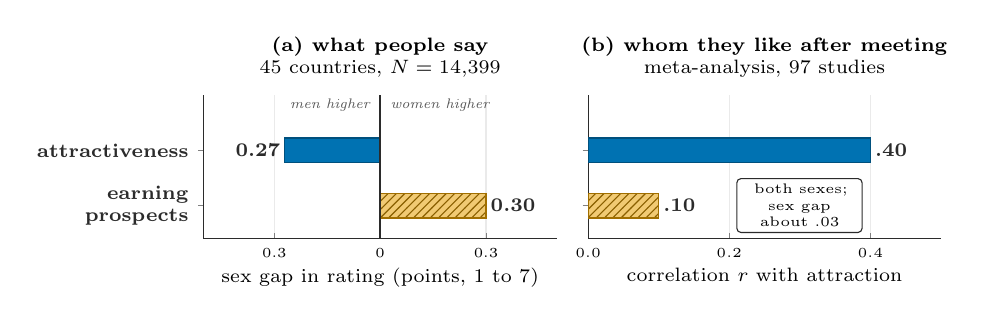
\begin{tikzpicture}[val/.style={font=\scriptsize\bfseries, text=hgink, inner sep=1.5pt}]
\begin{groupplot}[
  group style={group size=2 by 1, horizontal sep=4mm, yticklabels at=edge left},
  width=0.5\columnwidth, height=3.4cm,
  xbar, /pgf/bar width=9pt, /pgf/bar shift=0pt,
  ymin=0.4, ymax=3.0, ytick={1,2},
  yticklabels={earning\\prospects, attractiveness},
  yticklabel style={font=\scriptsize\bfseries, align=right, text=hgink},
  xticklabel style={font=\tiny, /pgf/number format/.cd, fixed, fixed zerofill, precision=1},
  title style={font=\scriptsize, align=center, yshift=-3pt},
  xlabel style={font=\scriptsize, yshift=3pt},
  axis lines*=left, axis line style={hgink}, xmajorgrids, grid style={hgink!10},
  major tick length=2pt, clip=false,
]
\nextgroupplot[
  title={\textbf{(a) what people say}\\45 countries, $N=14{,}399$},
  xmin=-0.5, xmax=0.5, xtick={-0.3,0,0.3}, xticklabels={0.3,0,0.3},
  xlabel={sex gap in rating (points, 1 to 7)},
]
\addplot[draw=hgorange!70!black, fill=hgorange!55, postaction={pattern=north east lines, pattern color=hgorange!60!black}]
  coordinates {(0.30,1)};
\addplot[draw=hgblue!70!black, fill=hgblue] coordinates {(-0.27,2)};
\node[val, anchor=west] at (axis cs:0.30,1) {0.30};
\node[val, anchor=east] at (axis cs:-0.27,2) {0.27};
\draw[hgink, thick] (axis cs:0,0.4) -- (axis cs:0,3.0);
\node[font=\tiny\itshape, text=hgink!80, anchor=north west, inner sep=1pt] at (axis cs:0.02,3.0) {women higher};
\node[font=\tiny\itshape, text=hgink!80, anchor=north east, inner sep=1pt] at (axis cs:-0.02,3.0) {men higher};
\nextgroupplot[
  title={\textbf{(b) whom they like after meeting}\\meta-analysis, 97 studies},
  xmin=0, xmax=0.5, xtick={0,0.2,0.4},
  xlabel={correlation $r$ with attraction},
]
\addplot[draw=hgorange!70!black, fill=hgorange!55, postaction={pattern=north east lines, pattern color=hgorange!60!black}]
  coordinates {(0.10,1)};
\addplot[draw=hgblue!70!black, fill=hgblue] coordinates {(0.40,2)};
\node[val, anchor=west] at (axis cs:0.10,1) {.10};
\node[val, anchor=west] at (axis cs:0.40,2) {.40};
\node[hgbadge, anchor=west, text width=1.45cm, font=\tiny] at (axis cs:0.21,1) {both sexes;\\sex gap about .03};
\end{groupplot}
\end{tikzpicture}

\caption{Stated versus revealed preferences. (a) In 45 countries, women rated a partner's financial prospects about 0.30 points higher than men did, and men rated physical attractiveness about 0.27 points higher (1 to 7 scale) \cite{walter2020}. (b) Once people have met, attractiveness predicts romantic evaluations at about $r=.40$ and earning prospects at about $r=.10$, for both sexes, with a sex difference near .03 \cite{eastwick2014} (read from an author copy). Values as reported; nothing is estimated here.}
\label{fig:stated}
\end{figure}

At first contact the difference comes back. Women on a US dating site weighted a man's income more than men weighted a woman's \cite{hitsch2010qme}. In a Tinder field experiment in Belgium (24 fake profiles, 3,600 evaluations), women strongly preferred highly educated men, while men showed neither a preference for nor an aversion to highly educated women \cite{neyt2019}. In speed dating, men did not value a woman's intelligence or ambition when it exceeded their own \cite{fisman2006}, a male-side asymmetry that also produces ``hypergamous'' couples. So status counts for more in screening and for much less once people actually meet.

\subsection{Actual Matching: Education (D1)}
The strongest pattern in marriage data is like marrying like. US educational homogamy rose from 1960 to 2003 \cite{schwartz2005}, and sorting on similarity runs through partner choice in general \cite{kalmijn1998}.

Educational hypergamy did exist: for most of the twentieth century, when spouses differed, he usually had more schooling. That pattern has reversed. Census data from 56 countries show a near-universal decline \cite{esteve2012}, and 420 samples from 120 countries (1960 to 2011) link the end of hypergamy to women overtaking men in education \cite{esteve2016}. In Western countries, couples in which the wife has more education now outnumber those in which the husband does \cite{vanbavel2018}. In the US, newlyweds moved from women marrying up (1980) to women marrying down (2008 to 2012) \cite{qian2017}. In Europe, highly educated women more often partnered with less educated men instead of staying single, and low-educated men more often stayed single \cite{dehauw2017}. Fig.~\ref{fig:reversal} sketches the shape of this change.

Two follow-ups matter for the online story. Marriages in which the wife had more education used to be more likely to end, but in recent US cohorts that link has gone \cite{schwartz2014}. And where a strong norm meets a changing supply, marriage can fall instead: in Japan, fewer highly educated women marry, which is linked to a shortage of men with the education and earnings they and the local norms expect \cite{raymo2005}.

\begin{figure}[t]
\centering
% Fig. 3: schematic of educational hypergamy reversing. ILLUSTRATIVE: the curves are
% hand-drawn logistic shapes, not data. Direction of change follows esteve2012,
% esteve2016, vanbavel2018, qian2017; no values are taken from any source.
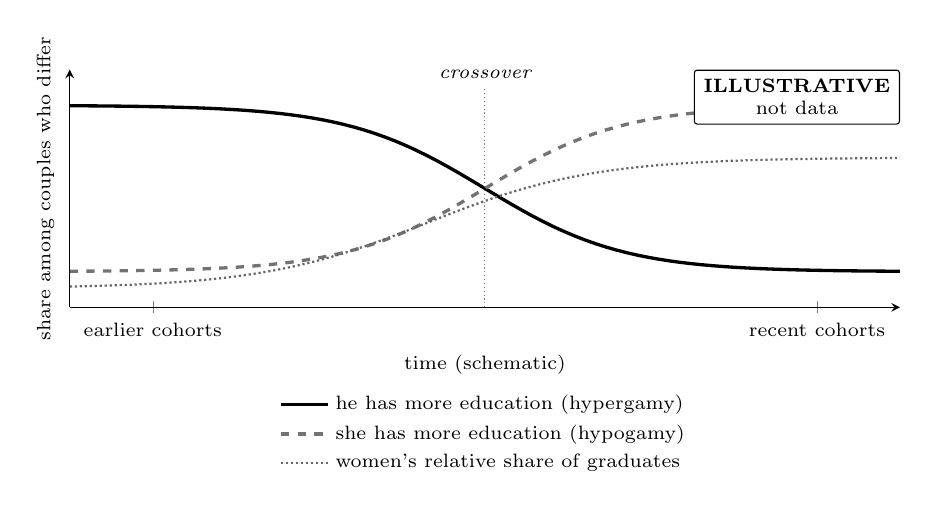
\begin{tikzpicture}
\begin{axis}[
  width=\columnwidth, height=4.6cm,
  xmin=0, xmax=10, ymin=0, ymax=1,
  xtick={1,9}, xticklabels={earlier cohorts, recent cohorts},
  ytick=\empty,
  xlabel={time (schematic)}, ylabel={share among couples who differ},
  ylabel style={font=\scriptsize}, xlabel style={font=\scriptsize},
  ticklabel style={font=\scriptsize},
  axis lines=left, clip=false,
  legend style={font=\scriptsize, draw=none, at={(0.5,-0.32)}, anchor=north, cells={anchor=west}},
  legend cell align=left,
]
\addplot[black, very thick, domain=0:10, samples=80] {0.15 + 0.7/(1+exp(1.2*(x-5)))};
\addlegendentry{he has more education (hypergamy)}
\addplot[black!55, very thick, dashed, domain=0:10, samples=80] {0.15 + 0.7/(1+exp(-1.2*(x-5)))};
\addlegendentry{she has more education (hypogamy)}
\addplot[black!60, densely dotted, thick, domain=0:10, samples=80] {0.08 + 0.55/(1+exp(-1.0*(x-4.3)))};
\addlegendentry{women's relative share of graduates}
\draw[black!50, densely dotted] (axis cs:5,0) -- (axis cs:5,0.92);
\node[font=\scriptsize\itshape, align=center, anchor=south] at (axis cs:5,0.92) {crossover};
\node[font=\scriptsize, draw, fill=white, rounded corners=1pt, anchor=north east, align=center]
  at (axis cs:10,1.0) {\textbf{ILLUSTRATIVE}\\not data};
\end{axis}
\end{tikzpicture}

\caption{Schematic of educational hypergamy reversing as women's education overtakes men's. \emph{Illustrative only}: the curves are drawn by hand and contain no data. The direction of change follows \cite{esteve2012,esteve2016,vanbavel2018,qian2017}. Timing and size vary by country.}
\label{fig:reversal}
\end{figure}

\subsection{Actual Matching: Income (D1)}
Income hypergamy outlived educational hypergamy. In the US, women's tendency to marry men with higher incomes persisted from 1980 to 2008--2012, and was \emph{stronger} when the wife was as educated as her husband or more \cite{qian2017}. In Swedish register data, women in education-hypogamous couples had higher class background and occupational prestige than their partners but lower income, partly because lower-earning people select into such couples \cite{chudnovskaya2020}. A partner who is ``up'' on one dimension is often ``down'' on another. Spouses' earnings have also become more alike over time, which is like-with-like again \cite{schwartz2010}.

The shortage side is real too. The men that unmarried US women would be expected to marry, constructed from the husbands of comparable married women, earn about 58\% more than the unmarried men actually available and are more often employed (90\% vs.\ 70\%) \cite{lichter2020}. When manufacturing declined, young men's earnings fell relative to women's and marriage fell with them \cite{autor2019}.

The best-known ``proof'' online is a sharp drop in the number of US couples just past the point where the wife out-earns the husband, read as a male-breadwinner norm \cite{bertrand2015}. Later work shows that matching models with no norm reproduce the distribution and that the drop comes from couples with exactly equal earnings \cite{binder2022}. In Finland it comes from co-working spouses whose earnings converge \cite{zinovyeva2021}, and a replication, not yet peer reviewed, finds the labour-force result turns to zero with hourly wages \cite{rosenberg2024}. The norm may exist, but this evidence does not settle it.

\subsection{Actual Matching: Age (D1)}
Age is the most stable finding. Women prefer and marry slightly older men at all ages, and men's preference for younger women grows as they age \cite{kenrick1992}. In the 45-country data, women's partners were on average 2.4 years older and men's 2.3 years younger, and the gap was smaller in more gender-equal countries \cite{walter2020}, the one place where equality clearly moderated a sex difference. In a Finnish sample ($N=2{,}655$), men's considered age range widened with age, but interest in much younger women was rarely turned into actual sex, because the other side chooses too \cite{antfolk2017}.

\subsection{Online Dating (D3)}
Meeting online became the most common way heterosexual US couples meet, overtaking meeting through friends around 2013 \cite{rosenfeld2019}, so app behaviour now matters for real couples.

On a large US site, desirability formed one shared hierarchy, and men and women both messaged people about 25\% more desirable than themselves (26\% and 23\%) \cite{bruch2018}. Men's desirability rose with education and peaked near age 50; women's fell from age 18 and peaked at an undergraduate degree. In six months of messages in one US city (8,259 men, 6,274 women), both sexes messaged the most desirable people regardless of their own standing; women sent four times fewer messages, but their messages were twice as likely to connect, and couple similarity arose mostly from unanswered messages \cite{kreager2014}. Feeding estimated preferences into Gale--Shapley matching \cite{gale1962} reproduces observed matches and marriage sorting \cite{hitsch2010aer}. Users also screen with a few deal-breakers before weighing anything else \cite{bruch2016}.


\begin{figure*}[t]
\centering
% Fig. 4: the Hypergamy Meter pipeline, drawn from app/src/model.rs and app/src/memes.rs.
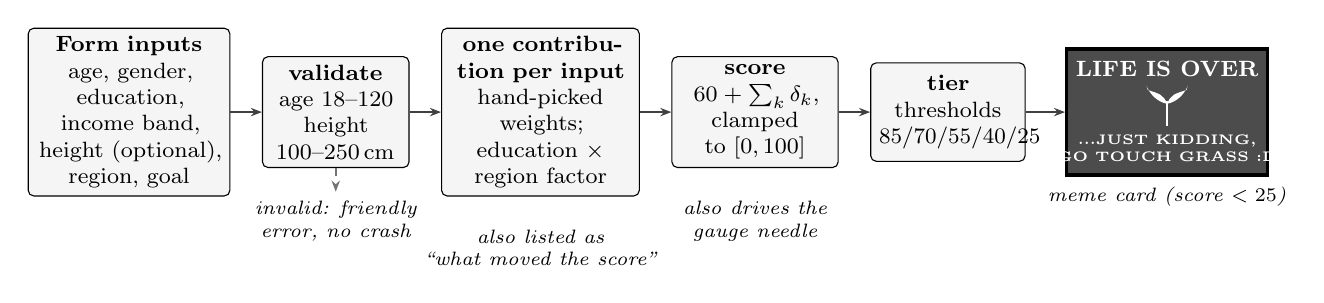
\begin{tikzpicture}[
  font=\footnotesize, node distance=4mm,
  box/.style={draw, rounded corners=2pt, align=center, fill=black!4, inner sep=3pt, minimum height=1.25cm},
  arr/.style={-{Stealth[length=4pt]}, thick, black!75},
]
\node[box, text width=2.35cm] (in) {\textbf{Form inputs}\\ age, gender, education, income band, height (optional), region, goal};
\node[box, text width=1.65cm, right=of in] (val) {\textbf{validate}\\ age 18--120\\ height 100--250\,cm};
\node[box, text width=2.3cm, right=of val] (con) {\textbf{one contribution per input}\\ hand-picked weights;\\ education $\times$ region factor};
\node[box, text width=1.9cm, right=of con] (sc) {\textbf{score}\\ $60+\sum_k \delta_k$,\\ clamped to $[0,100]$};
\node[box, text width=1.75cm, right=of sc] (tier) {\textbf{tier}\\ thresholds\\ 85/70/55/40/25};
% meme card
\node[right=5mm of tier, draw, very thick, fill=black!70, minimum width=2.55cm, minimum height=1.6cm] (card) {};
\node[font=\bfseries\footnotesize, text=white, anchor=north] at ([yshift=-1.5pt]card.north) {LIFE IS OVER};
% seedling, standing in for the app's emoji
\draw[white, thick] ([yshift=-5pt]card.center) -- ([yshift=4pt]card.center);
\fill[white] ([yshift=3pt]card.center) .. controls +(-0.25,0.05) and +(-0.05,0.18) .. ([xshift=-7pt,yshift=8pt]card.center) .. controls +(0.15,-0.05) and +(-0.05,0.12) .. ([yshift=3pt]card.center);
\fill[white] ([yshift=3pt]card.center) .. controls +(0.25,0.05) and +(0.05,0.18) .. ([xshift=7pt,yshift=8pt]card.center) .. controls +(-0.15,-0.05) and +(0.05,0.12) .. ([yshift=3pt]card.center);
\node[font=\bfseries\tiny, text=white, anchor=south, align=center] at ([yshift=2pt]card.south) {...JUST KIDDING,\\ GO TOUCH GRASS :D};
\node[font=\scriptsize\itshape, anchor=north, align=center] at (card.south) {meme card (score $<25$)};
\draw[arr] (in) -- (val);
\draw[arr] (val) -- (con);
\draw[arr] (con) -- (sc);
\draw[arr] (sc) -- (tier);
\draw[arr] (tier) -- (card);
\node[font=\scriptsize\itshape, anchor=north, align=center] (err) at ([yshift=-3mm]val.south) {invalid: friendly\\error, no crash};
\draw[arr, dashed, black!55] (val.south) -- (err.north);
\node[font=\scriptsize\itshape, anchor=north, align=center] at ([yshift=-3mm]con.south) {also listed as\\``what moved the score''};
\node[font=\scriptsize\itshape, anchor=north, align=center] at ([yshift=-3mm]sc.south) {also drives the\\gauge needle};
\end{tikzpicture}

\caption{The Hypergamy Meter pipeline, as implemented in \texttt{app/src/model.rs} and \texttt{app/src/memes.rs}. Every step is a pure function. The two cards are the lowest-tier memes for men and for women (non-binary users get ``IT'S OVER (ALL GENDERS EDITION)''). The weights are illustrative, not estimates.}
\label{fig:pipeline}
\end{figure*}

\subsection{The 80/20 Claim (D4)}
\begin{figure}[t]
\centering
% Fig.: "everyone aims up". DATA from bruch2018 (full text): on a large US dating site, men
% messaged partners about 26% and women about 23% more desirable than themselves.
% Arrow length is proportional to the percentage. Greyscale: men = solid dark blue,
% women = vermilion with hatching; both arrows are also labelled.
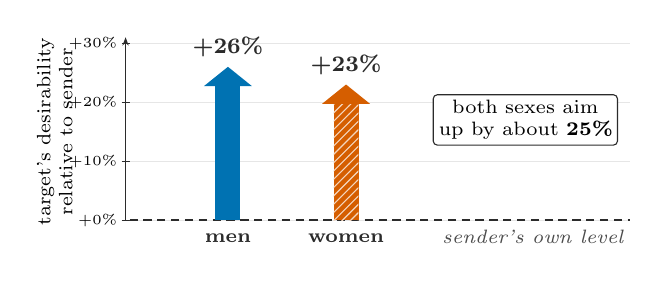
\begin{tikzpicture}[
  x=1cm, y=0.075cm,
  up/.style={line width=9pt, -{Triangle[width=17pt, length=7pt]}},
  num/.style={font=\footnotesize\bfseries, text=hgink},
  who/.style={font=\scriptsize\bfseries, text=hgink, anchor=north},
]
% scale
\draw[hgink, -{Stealth[length=3pt]}] (0,0) -- (0,31);
\foreach \v in {0,10,20,30} {
  \draw[hgink] (-0.05,\v) -- (0.05,\v);
  \node[font=\tiny, anchor=east, inner sep=1.5pt] at (-0.05,\v) {+\v\%};
  \draw[hgink!12] (0.05,\v) -- (6.4,\v);
}
\node[font=\scriptsize, rotate=90, anchor=south, align=center] at (-0.55,15) {target's desirability\\relative to sender};
% own level
\draw[hgink, thick, densely dashed] (0.05,0) -- (6.4,0);
\node[font=\scriptsize\itshape, anchor=north west, text=hgink!85] at (3.9,0) {sender's own level};
% arrows: men 26%, women 23% (arrow tip ends at the value)
\draw[up, hgblue] (1.3,0) -- (1.3,26);
\draw[up, hgverm] (2.8,0) -- (2.8,23);
\fill[pattern=north east lines, pattern color=white!75!hgverm] (2.8-0.158,0) rectangle (2.8+0.158,19.6);
\node[num, anchor=south] at (1.3,26) {+26\%};
\node[num, anchor=south] at (2.8,23) {+23\%};
\node[who] at (1.3,-0.6) {men};
\node[who] at (2.8,-0.6) {women};
% verdict
\node[hgbadge, anchor=west, text width=2.2cm, font=\scriptsize] at (3.9,17)
  {both sexes aim up by about \textbf{25\%}};
\end{tikzpicture}

\caption{Everyone aims up. On a large US dating site, men messaged partners about 26\% and women about 23\% more desirable than themselves \cite{bruch2018}. Arrow length is proportional to the reported value. Aiming up is not a female trait.}
\label{fig:aimup}
\end{figure}

The claim is that most women compete for the top fifth of men. The best research figure on swipe asymmetry is small: in a conference study of Tinder activity by fake profiles, men matched about 0.6\% of the time and women about 10\% \cite{tyson2016}, as reported in secondary summaries. Popular ``Gini of likes'' figures come from an anonymous blog post and from company numbers quoted in the press; we could not audit them and do not cite them.

The peer-reviewed data tell a different story. Attention is unequal for both sexes and men get fewer replies, but both sexes aim above themselves by about the same amount (Fig.~\ref{fig:aimup}), women's messages are not limited to a top 20\%, and final couples are mostly matched like with like \cite{bruch2018,kreager2014}. Even OkCupid's 2009 post, a likely root of the ``women rate 80\% of men below average'' line, reported that women's messaging was only slightly skewed toward attractive men \cite{rudder2009}. Attention inequality on one app is not partnering inequality in a population. Verdict: not supported as stated.

\section{Beyond Status}
\label{sec:beyond}
Online arguments about dating go well past money and degrees: casual versus serious dating, height, build, penis size, intelligence, personality, looks, age, race and even paternity and genetics. Tables~\ref{tab:beyond} and~\ref{tab:darkpat} give the verdicts on the same scale as Table~\ref{tab:verdict}. One warning applies to most of it. Much of this evidence comes from small groups of Western students rating photos, figures or questionnaires, so it measures stated or first-impression preferences (D2, or D3 at first contact). Where data on real contacts or couples exist, the effects are usually smaller.


\begin{table*}[!t]
\centering
\caption{Verdicts beyond status, same symbols and strength scale as Table~\ref{tab:verdict}. In the Def.\ column, -- marks a claim outside D1 to D4. $^\dagger$At least one source in the row was read only in a secondary summary or in metadata (see Limitations).}
\label{tab:beyond}
\scriptsize
\renewcommand{\arraystretch}{1.07}
\setlength{\tabcolsep}{4pt}
\begin{tabular}{@{}>{\raggedright\arraybackslash}p{5.85cm} c c >{\raggedright\arraybackslash}p{4.5cm} l >{\raggedright\arraybackslash}p{2.9cm}@{}}
\toprule
\textbf{Claim} & \textbf{Def.} & & \textbf{Verdict} & \textbf{Strength} & \textbf{Main sources}\\
\midrule
\rowcolor{black!6}
Women weight status more for long-term partners; for short-term partners both sexes put looks first & D2 & \vexists & exists, in stated preferences & moderate & \cite{buss1993,kenrick1990,likenrick2006,braun2006}\\
Men lower their standards for casual sex far more than women, but not for a long-term partner & D2 & \vexists & exists (stated) & moderate & \cite{kenrick1990,buss1993}\\
\rowcolor{black!6}
Women's taste shifts toward masculine men around ovulation & D2 & \vnot & mostly not: meta-analyses disagree, large preregistered studies find no shift & moderate & \cite{gildersleeve2014,wood2014,jones2018,stern2020}\\
Women want taller men more than men want shorter women & D2, D3 & \vexists & exists, stated and at first contact & strong & \cite{stulp2013paid,hitsch2010qme}$^\dagger$\\
\rowcolor{black!6}
Couples follow the ``man taller'' norm & D1 & \vpartly & yes, but only a little more often than chance & strong & \cite{stulp2013plos}\\
Tall men get far more messages (``6'3'' gets 65\% more than 5'7''\,'') & D3 & \vunclear & height counts relative to one's own; the 65\% is from an unpublished draft & weak & \cite{hitsch2010qme,xia2014}$^\dagger$\\
\rowcolor{black!6}
Perceived upper-body strength drives ratings of men's bodies & D2 & \vexists & exists in photo and figure ratings & moderate & \cite{sell2017,mautz2013,frederick2007,braun2006}\\
Arm span (``wingspan'') affects attractiveness & -- & \vunclear & no direct study; it would mostly be a height effect & none & \cite{sorokowski2008} (proxy)$^\dagger$\\
\rowcolor{black!6}
Penis size affects women's ratings of men & D2 & \vpartly & small, about as large as height, diminishing returns & weak to moderate & \cite{mautz2013,prause2015}$^\dagger$\\
Women prefer a larger penis for short-term partners & D2 & \vpartly & 0.3\,cm difference in one study & weak & \cite{prause2015}\\
\rowcolor{black!6}
Men overestimate how much size matters to women & D2 & \vexists & 85\% of women satisfied vs.\ 55\% of men & moderate & \cite{lever2006}\\
Intelligence is among the most wanted traits for both sexes & D2 & \vexists & exists & strong & \cite{buss1989,walter2020}\\
\rowcolor{black!6}
Wanting intelligence has a ceiling near the 90th percentile & D2 & \vpartly & found twice, one lab, stated ratings only & weak to moderate & \cite{gignac2018,gignac2019}$^\dagger$\\
Partners resemble each other in intelligence and education & D1 & \vexists & $r\approx.44$ for IQ, $.55$ for education & strong & \cite{horwitz2023}\\
\rowcolor{black!6}
Higher intelligence helps people find a partner & D1 & \vunclear & one old cohort, opposite signs by sex & weak & \cite{taylor2005}$^\dagger$\\
Looks drive online messages for both sexes, a bit more for men & D3 & \vexists & exists & strong & \cite{hitsch2010qme,eastwick2014,lee2008}\\
\rowcolor{black!6}
People rated less attractive adjust whom they approach, men less than women & D3 & \vexists & exists & moderate & \cite{lee2008,kreager2014}\\
Men's messages target younger women, more so as men age & D3 & \vexists & exists & moderate to strong & \cite{hitsch2010qme,skopek2011age,bruch2018}\\
\rowcolor{black!6}
A measured ``Gini of likes'' shows extreme inequality for men & D4 & \vunclear & no peer-reviewed or audited estimate & weak (grade D) & \cite{tyson2016}$^\dagger$\\
Racial hierarchies shape who is contacted and answered & D3 & \vexists & exists, as documented bias & strong & \cite{lin2013,robnett2011,hitsch2010qme,bruch2019,curington2021}$^\dagger$\\
\rowcolor{black!6}
Racial bias in dating is fading & D1, D3 & \vunclear & intermarriage rising for some groups only & weak to moderate & \cite{qian2011,rudder2014race}$^\dagger$\\
\bottomrule
\end{tabular}
\end{table*}

\begin{table*}[!t]
\centering
\caption{Verdicts on personality and paternity, same symbols and strength scale as Table~\ref{tab:verdict}. -- marks a claim outside D1 to D4. $^\dagger$At least one source in the row was read only in a secondary summary or in metadata (see Limitations).}
\label{tab:darkpat}
\scriptsize
\renewcommand{\arraystretch}{1.1}
\setlength{\tabcolsep}{4pt}
\begin{tabular}{@{}>{\raggedright\arraybackslash}p{5.85cm} c c >{\raggedright\arraybackslash}p{4.5cm} l >{\raggedright\arraybackslash}p{2.9cm}@{}}
\toprule
\textbf{Claim} & \textbf{Def.} & & \textbf{Verdict} & \textbf{Strength} & \textbf{Main sources}\\
\multicolumn{6}{@{}l}{\textit{Personality: the Dark Triad (Section~\ref{sec:darktriad})}}\\
\rowcolor{black!6}
Narcissism and psychopathy go with more casual sex and more partners & -- & \vexists & exists (self-reported), both sexes, in 53 nations, stronger in men & moderate to strong & \cite{borrazleon2021,schmitt2017narc,lee2013sex,jonason2009,freyth2023}\\
The short-term link is a male pattern & -- & \vnot & no: in women it runs through psychopathy & moderate & \cite{freyth2023,borrazleon2021,jauk2016}\\
\rowcolor{black!6}
Men score higher on the Dark Triad & -- & \vexists & small to moderate (narcissism $d=.26$), large overlap & strong & \cite{muris2017,grijalva2015,jonason2020countries}\\
Narcissists are chosen more in real first meetings & D3 & \vexists & both sexes (street approaches, speed dating, first sight), mostly through looks and boldness & moderate & \cite{dufner2013,jauk2016,back2010,holtzman2010,holtzman2013}$^\dagger$\\
\rowcolor{black!6}
Women rate a fictional ``dark'' man as more attractive & D2 & \vpartly & mixed: yes for written profiles and short-term ``cads''; no for faces and in the largest randomised study & weak to moderate & for: \cite{carter2014,aitken2013,haslam2015}; against: \cite{brewer2018faces,lyons2016faces,dragostinov2025}$^\dagger$\\
Dominance makes men more attractive & D2 & \vpartly & confidence yes; dominance alone adds little without kindness & moderate & \cite{sadalla1987,jensencampbell1995,burger1999,snyder2008}$^\dagger$\\
\rowcolor{black!6}
Machiavellian and psychopathic traits are attractive in themselves & D2 & \vnot & mostly not, except to raters who score high themselves & moderate & \cite{rauthmann2013,dragostinov2025,jonason2015birds,watts2019,marcinkowska2015}$^\dagger$\\
The narcissist's appeal fades with acquaintance & -- & \vexists & among strangers over weeks; not tested in dating couples & moderate & \cite{paulhus1998,leckelt2015}$^\dagger$\\
\rowcolor{black!6}
Dark Triad partners are preferred for the long term & D2 & \vnot & does not exist in any rating study & moderate & \cite{jonason2015birds,dragostinov2025,aitken2013}$^\dagger$\\
Dark Triad traits predict infidelity, poaching and lower satisfaction & -- & \vexists & small effects (infidelity $r=.13$ to $.25$), both sexes & moderate & \cite{ataman2025,jonason2010poach,brewer2015,kardum2024}$^\dagger$\\
\rowcolor{black!6}
``Nice guys finish last'' & D3 & \vpartly & true for partner counts, false for being chosen as a partner & moderate & \cite{herold1999,urbaniak2003,mcdaniel2005,jensencampbell1995}$^\dagger$\\
``Women love bad boys'' & D2, D3 & \vpartly & split: yes for flings and first meetings when ``bad'' means bold and self-promoting; no long term; men show the same pattern toward narcissistic women & moderate & see Section~\ref{sec:darktriad}\\
\midrule
\multicolumn{6}{@{}l}{\textit{Paternity and Y-chromosome history (Section~\ref{sec:paternity})}}\\
\rowcolor{black!6}
10 to 30\% of children are not fathered by the presumed father & -- & \vnot & about 1 to 2\% in populations; about 30\% only among men who doubted and tested & strong & \cite{anderson2006,larmuseau2013,larmuseau2019,greeff2015,dahlen2022,bellis2005}$^\dagger$\\
Misattributed paternity is higher in poorer, younger, unmarried or dense urban settings & -- & \vexists & exists & moderate & \cite{bellis2005,larmuseau2019,dahlen2022}\\
\rowcolor{black!6}
Misattributed paternity rate in France & -- & \vunclear & no peer-reviewed estimate; tests only by court order; neighbours about 1 to 2\% & none for France & \cite{larmuseau2013,larmuseau2019}\\
Historically, fewer men than women passed on their genes & -- & \vexists & exists: long-run female effective size about twice the male & strong & \cite{wilder2004,karmin2015,poznik2016,batini2015}\\
\rowcolor{black!6}
``17 women reproduced for every man'' & -- & \vexists & exists as an effective-size ratio (peak, 8,000 to 4,000 years ago); not a head count & moderate & \cite{karmin2015}\\
The male bottleneck was caused by women choosing few men & -- & \vunclear & debated: polygyny and inherited status (including female choice), clan competition, conquest and migration & moderate & \cite{karmin2015,zeng2018,poznik2016,batini2015}\\
\rowcolor{black!6}
``Twice as many women as men reproduced''; ``80\% of women, 40\% of men'' & -- & \vpartly & the 2:1 is measured (moderate); the 80/40 is an illustration (weak) & moderate / weak & \cite{wilder2004,karmin2015,baumeister2010}$^\dagger$\\
Haplogroup N1c is very common among Finnish and Baltic men & -- & \vexists & Finland 58 to 64\%, Latvia 42\%, Lithuania 37\%, Estonia 31\% & strong & \cite{rootsi2007,preussner2025,ilumae2016}\\
\rowcolor{black!6}
That frequency reflects outsized male-line success of a few founders & -- & \vexists & over about 5,000 years, with migration, founder effects and drift & moderate & \cite{ilumae2016,rootsi2007,lappalainen2008,batini2015}\\
A common haplogroup shows that a few living men father most children today & -- & \vnot & does not exist & moderate & \cite{ilumae2016,pliss2015}\\
\bottomrule
\end{tabular}
\end{table*}

\subsection{Short-Term Versus Long-Term Partners}
Sexual strategies theory holds that both sexes pursue separate strategies for casual and committed relationships \cite{buss1993,buss2019}, and stated preferences agree. When 93 US students set minimum standards on 24 traits for four levels of commitment, women were more selective overall, especially on status. Men accepted far lower standards for a sexual partner but were nearly as choosy as women for a long-term one \cite{kenrick1990}. In mate-budget tasks women treated status as a necessity for a long-term partner, while for a short-term partner both sexes spent first on looks \cite{likenrick2006}, and body shape mattered most for a one-time encounter \cite{braun2006}. In a German community speed-dating study ($N=382$, ages 18 to 54), both sexes chose mainly on looks and women also on men's education and income. Only 6\% of matches led to sex and 4\% to a relationship within a year \cite{asendorpf2011}.

The ovulation story, that women prefer more masculine men around ovulation, has not held up. Two meta-analyses of the same literature disagree \cite{gildersleeve2014,wood2014}. The largest longitudinal study ($N=584$, hormone measures) found no link between hormones and a preference for masculine faces \cite{jones2018}, and a preregistered study with ovulation tests ($N=157$) found no shift \cite{stern2020}. Both still found that masculinity counts more in short-term ratings. So context matters and the cycle mostly does not. The stated status preference is mainly a long-term one, and one status weight for every kind of relationship overstates hypergamy for casual dating.

\subsection{Height and Build}
Women want a taller partner more than men want a shorter one: in a Dutch student sample ($N=650$), women were most satisfied with a partner about 21\,cm taller, men with one about 8\,cm shorter \cite{stulp2013paid}. On a US dating site the effect at first contact was relative to one's own height, and women showed no preference for absolute height \cite{hitsch2010qme}. The famous ``6'3'' gets 65\% more messages than 5'7''\,'' comes from a 2006 draft of that work, and the published papers say non-robust earlier results were dropped. Profile heights are also inflated, mostly by men \cite{hancock2007}. In 12,502 UK couples, partners' heights correlated at $r=.18$, and the man was not taller in 7.5\% of couples against 10.2\% expected under random pairing \cite{stulp2013plos} (Fig.~\ref{fig:taller}). Random pairing alone would give the ``man taller'' norm about 90\% of the time, because men are taller on average.

\begin{figure}[t]
\centering
% Fig.: the "man taller" norm. DATA from stulp2013plos (abstract and full text): in 12,502
% UK couples the man was not taller in 7.5% of couples, against 10.2% expected under random
% pairing. Only those two values are printed; each bar is drawn to 100%.
% Greyscale: "man taller" = solid dark blue, "man not taller" = light orange + hatching.
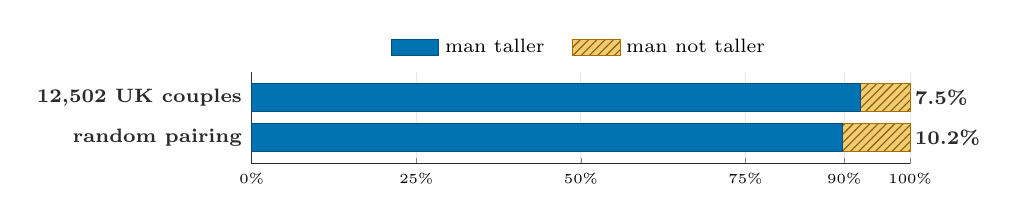
\begin{tikzpicture}
\begin{axis}[
  width=0.82\columnwidth, height=2.75cm,
  xbar stacked, bar width=10pt,
  xmin=0, xmax=100, xtick={0,25,50,75,90,100},
  xticklabel={\pgfmathprintnumber{\tick}\%},
  xticklabel style={font=\tiny},
  ymin=0.35, ymax=2.65, ytick={1,2},
  yticklabels={random pairing,{12,502 UK couples}},
  yticklabel style={font=\scriptsize\bfseries, text=hgink, align=right},
  axis lines*=left, axis line style={hgink}, xmajorgrids, grid style={hgink!12},
  major tick length=2pt, clip=false,
  legend style={font=\scriptsize, at={(0.5,1.04)}, anchor=south, draw=none, legend columns=2,
    /tikz/every even column/.append style={column sep=8pt}}, area legend,
]
\addplot[draw=hgblue!70!black, fill=hgblue] coordinates {(89.8,1) (92.5,2)};
\addplot[draw=hgorange!70!black, fill=hgorange!55, postaction={pattern=north east lines, pattern color=hgorange!60!black}]
  coordinates {(10.2,1) (7.5,2)};
\legend{man taller, man not taller}
\node[font=\scriptsize\bfseries, text=hgink, anchor=west, inner sep=1.5pt] at (axis cs:100,1) {10.2\%};
\node[font=\scriptsize\bfseries, text=hgink, anchor=west, inner sep=1.5pt] at (axis cs:100,2) {7.5\%};
\end{axis}
\end{tikzpicture}

\caption{The ``man taller'' norm in 12,502 UK couples: the man was not taller in 7.5\% of couples, against 10.2\% expected under random pairing \cite{stulp2013plos}. The norm holds only a little more often than chance, which alone gives it about 90\% of the time. Each bar adds up to 100\%.}
\label{fig:taller}
\end{figure}

For men's bodies, perceived upper-body strength explained over 70\% of the variation in rated bodily attractiveness \cite{sell2017}. Women rated muscular men as sexier but less committed and rated moderate muscularity highest \cite{frederick2007}, and torso shape was the strongest predictor for life-size male figures \cite{mautz2013}. We found no study on arm span. The nearest proxy is leg length, where legs about 5\% longer than average were rated most attractive \cite{sorokowski2008}. All of this is ratings of photos and figures, not real partner choice.

\subsection{Penis Size}
In ratings of life-size figures, larger size raised attractiveness with diminishing returns, about as much as height and less than torso shape \cite{mautz2013}. With 3D models, 75 US women preferred about 16.3\,cm length for a one-time partner and 16.0\,cm for a long-term one \cite{prause2015}. Clinician-measured studies of up to 15,521 men give a mean erect length of 13.1\,cm (SD 1.7) \cite{veale2015}, though handled models and clinical measurements are not directly comparable. In an online survey of 52,031 heterosexual US adults, 85\% of women were satisfied with their partner's size, but only 55\% of men with their own \cite{lever2006}. Size worries men far more than it matters to women, and no study links it to actual partner choice.

\subsection{Intelligence}
Intelligence ranks near the top for both sexes \cite{buss1989,walter2020}. Rated desirability of a partner's IQ peaked around the 90th percentile (about IQ 120) and dropped slightly at the 99th \cite{gignac2018}, and a replication with 214 young adults found the same \cite{gignac2019}. Both are stated ratings from one lab. Couples are clearly matched: a meta-analysis of 199 studies gives partner correlations of $r=.44$ for IQ and $r=.55$ for education \cite{horwitz2023}. Whether intelligence helps anyone find a partner is unclear. In a Scottish cohort born in 1921 ($N=883$), higher childhood IQ lowered women's odds of marrying by mid-life (odds ratio 0.42 per standard deviation), while the link for men was positive but not significant \cite{taylor2005}.

\subsection{Personality: Do ``Bad Boys'' Win?}
\label{sec:darktriad}
The Dark Triad is three overlapping traits: narcissism (grandiosity, entitlement), Machiavellianism (cynical manipulation) and psychopathy (callousness, impulsivity) \cite{paulhus2002}. The studies measure subclinical levels with short questionnaires, mostly in students and online panels, and most are cross-sectional self-reports \cite{muris2017}. Men score higher on average \cite{muris2017}. For narcissism the gap is $d=.26$ across 470,846 people \cite{grijalva2015}, so many women score above the average man. Online, a ``bad boy'' mixes confidence, dominance, risk-taking and low agreeableness, and the answer differs by piece (Table~\ref{tab:darkpat}).

\textbf{Partner counts: exists.} People higher in narcissism and psychopathy report more sexual partners, in men and in women analysed separately \cite{borrazleon2021}. The traits go with casual sex but not with long-term mating, more strongly in men \cite{jonason2009,lee2013sex}, and the narcissism link held in all 11 world regions of a 30,470-person survey \cite{schmitt2017narc}. In 495 people, Machiavellianism carried the link in men and psychopathy in women, and women high in psychopathy reported more partners and more one-night stands \cite{freyth2023}. The counts are self-reported, narcissists over-claim, and more partners is not more children.

\textbf{Real first meetings: exists.} In a field study, more narcissistic men obtained more contact details from women they approached in the street, and across three studies narcissism raised short-term appeal through looks and social boldness \cite{dufner2013}. In speed dating (90 adults, 691 dates), narcissism predicted being chosen in both sexes, through looks in women and extraversion in men. Once looks were controlled, no Dark Triad effect remained \cite{jauk2016}. Narcissists are also more popular at first sight among strangers \cite{back2010}, partly through grooming \cite{holtzman2010,holtzman2013}.

\textbf{Fictional profiles: mixed.} For: 128 female students (mean age 19) rated a written high Dark Triad man more attractive than a control, 4.44 against 3.34 on a 6-point scale, $d=0.94$, partly because he also seemed more extraverted \cite{carter2014}. Women preferred high-Machiavellian ``cads'' for short-term and low-Machiavellian ``dads'' for long-term partners \cite{aitken2013}, and women who wanted to marry, like women with many past partners, found narcissistic traits more attractive \cite{haslam2015}. Against: women disliked composite faces high in each trait, short- and long-term \cite{brewer2018faces,lyons2016faces}, and older women reportedly preferred the low version \cite{qureshi2016}. In the largest test ($N=794$, faces decoupled from the text) both sexes preferred low levels for both flings and long-term partners \cite{dragostinov2025}.

\textbf{Dominance: partly.} Dominant, but not aggressive, behaviour raised men's sexual attractiveness \cite{sadalla1987}. Later work found that dominance alone added nothing without kindness \cite{jensencampbell1995}, that both dominant and non-dominant men lost appeal against a neutral control \cite{burger1999}, and that women preferred prestige to dominance except in athletic competition and for a short-term partner \cite{snyder2008}.

\textbf{Callousness as such: mostly does not exist.} Most raters dislike Machiavellian and psychopathic targets \cite{rauthmann2013,watts2019}. The exception is raters who score high themselves or are open to casual sex \cite{jonason2015birds,watts2019,marcinkowska2015}, and couples resemble each other on all three traits \cite{richards2024}.

\textbf{Long term: does not exist.} No rating study prefers high scorers as long-term partners \cite{jonason2015birds,dragostinov2025}. The narcissist's appeal fades among strangers who meet weekly \cite{paulhus1998,leckelt2015}. High scorers poach partners more and leave more often \cite{jonason2010poach}. Infidelity correlated with narcissism at $r=.13$, Machiavellianism at $r=.23$ and psychopathy at $r=.25$ in a meta-analysis of 11 studies \cite{ataman2025}, women's scores predicted their own infidelity \cite{brewer2015}, and in 205 couples dark traits lowered both partners' satisfaction \cite{kardum2024}.

\textbf{Nice guys finish last: partly.} In partner counts, yes. More than half of 165 Canadian university women agreed that nice guys have fewer partners, and women with more partners picked the bad boy more often \cite{herold1999}. For casual sex, looks counted more than niceness \cite{urbaniak2003}. As a partner, no. Most of the same women preferred the nice guy as a date \cite{herold1999}, prosocial men were rated more desirable \cite{jensencampbell1995}, and women chose the nice guy for commitment \cite{mcdaniel2005}.

\textbf{Verdict: split.} ``Women love bad boys'' is true for flings, first meetings and partner counts, when ``bad'' means bold, good-looking and self-promoting. It is false for long-term choice and mostly false for callousness and manipulation. Men show the same pattern toward narcissistic women, who are also chosen more at first meetings \cite{jauk2016}.

\subsection{The Famous Dating-App Numbers}
Looks drive first contact for both sexes, a bit more for men \cite{hitsch2010qme,lee2008}, and men's messages target younger women, more so as they age \cite{hitsch2010qme,skopek2011age}. Table~\ref{tab:appnums} grades the numbers that circulate in the debate. The peer-reviewed ones say that both sexes aim up and that markets split by age and race \cite{bruch2018,bruch2019,hitsch2010qme}. The most quoted ones (the Tinder and Hinge ``Gini of likes'', ``women rate 80\% of men below average'', ``6'3'' gets 65\% more'') come from blogs, press retellings or a dropped draft. We found no peer-reviewed or audited estimate of like or swipe inequality on a swipe app. Unequal attention on apps is plausible and fits the messaging studies, but every specific ``Gini'' or ``80/20'' number is blog-grade.

\begin{table}[t]
\centering
\caption{Famous dating-app figures by evidence grade: A peer-reviewed and large or replicated, C conference paper, draft or book, D company blog, anonymous post or press.}
\label{tab:appnums}
\footnotesize
\renewcommand{\arraystretch}{1.1}
\begin{tabular}{@{}>{\raggedright\arraybackslash}p{4.25cm}>{\raggedright\arraybackslash}p{2.75cm}c@{}}
\toprule
\textbf{Figure} & \textbf{Source} & \textbf{Grade}\\
\midrule
Both sexes message about 25\% ``up'' & \cite{bruch2018} & A\\
Women weight income, men looks, a bit more & \cite{hitsch2010qme} & A\\
Markets split by age and race & \cite{bruch2019} & A\\
Tinder matches: men about 0.6\%, women about 10\% & \cite{tyson2016} & C\\
6'3'' men get 65\% more messages than 5'7'' & 2006 draft, dropped from \cite{hitsch2010qme} & C\\
Women rate 80\% of men below medium & OkCupid blog \cite{rudder2009} & D\\
Racial attraction charts, 2009 to 2014 & OkCupid blog \cite{rudder2014race} & D\\
Tinder ``Gini of likes'' 0.58 & anonymous blog post (not cited) & D\\
Hinge Gini for men 0.54 or 0.73 & press retellings, which disagree (not cited) & D\\
\bottomrule
\end{tabular}
\end{table}

\subsection{Race and Ethnicity: Documented Bias}
This subsection describes discrimination. It does not rank anyone's worth. On US dating sites both sexes mostly contact people of their own race, and 30 of 31 estimated race effects were negative. A white man was 10\% less likely to contact a black woman than a white woman, and a white woman 12\% less likely to contact an Asian man than a white man \cite{hitsch2010qme}. In replies a racial hierarchy appeared that a college degree did not offset \cite{lin2013}. In 6,070 US profiles, Asian men and black women were the most excluded \cite{robnett2011}. A book-length study calls this ``digital-sexual racism'' \cite{curington2021}. OkCupid's blog charts point the same way, with no decline from 2009 to 2014 by the company's account \cite{rudder2014race}. In US marriages, black-white intermarriage tripled between 1980 and 2008, while intermarriage with whites stalled for Asians and American Indians \cite{qian2011}. These studies measure bias against people, not anyone's value as a partner, which is why the app in Section~\ref{sec:app} has no ethnicity input.

\subsection{Paternity and Y-Chromosome History}
\label{sec:paternity}
Two genetic claims circulate online: that 10 to 30\% of children are not their presumed father's, as proof of a female ``dual strategy'' (commit to a provider, conceive with someone else), and that far fewer men than women have had children. The first fails as a population figure. The second holds, but its cause is debated.

\textbf{``10 to 30\% of children are not their father's.''} Population studies put the rate far lower (Fig.~\ref{fig:paternity}). Y-chromosome typing combined with genealogies gives about 1 to 2\% per generation in Flanders \cite{larmuseau2013} and 0.9\% (95\% CI 0.4 to 1.5\%) over 330 years in 23 Afrikaner families \cite{greeff2015}. Swedish blood-group data on nearly two million families give 1.7\%, falling to about 1\% today \cite{dahlen2022}. A review of 67 studies found 1.7 to 1.9\% among men confident of their paternity and about 30\% among men who doubted it and paid for a test \cite{anderson2006}. That 30\% comes from a press release, unchecked against the paper. It is real, but it describes a group selected for suspicion. A review that pools both kinds of sample reports 0.8 to 30\%, median 3.7\% \cite{bellis2005}. Context matters. Among married couples in the Low Countries the rate ranged from 0.4\% to 5.9\% over 500 years, highest among poor families in crowded late-19th-century cities \cite{larmuseau2019}, and it is higher for younger, deprived, cohabiting \cite{bellis2005} and less educated parents \cite{dahlen2022}. A historical rate near 1\% argues against the idea that women routinely seek other men's genes while staying with a provider \cite{larmuseau2016}.

\begin{figure}[t]
\centering
% Fig.: viral misattributed-paternity claim vs measured rates. DATA from ../notes.md:
% greeff2015 0.9% (95% CI 0.4-1.5%), larmuseau2013 about 1-2% per generation,
% larmuseau2019 0.4-5.9% (married couples, 500 years), dahlen2022 1.7% (Sweden),
% anderson2006 1.7-1.9% (high paternity confidence, abstract) and about 30% (men who doubted
% and tested; secondary, press release). The 10-30% band is the online claim.
% Greyscale: claim = hatched light band; population = dark (blue) dots and bars;
% selected sample = light (orange) square with a direct label.
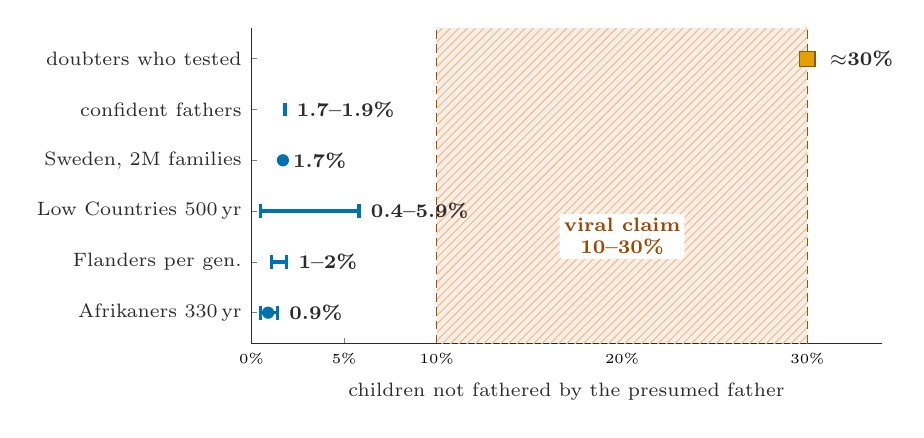
\begin{tikzpicture}
\begin{axis}[
  width=0.66\columnwidth, height=4.0cm, scale only axis,
  xmin=0, xmax=34, xtick={0,5,10,20,30},
  xticklabel={\pgfmathprintnumber{\tick}\%}, xticklabel style={font=\tiny},
  xlabel={children not fathered by the presumed father}, xlabel style={font=\scriptsize, text=hgink},
  ymin=0.4, ymax=6.6, ytick={1,...,6},
  yticklabels={Afrikaners 330\,yr, Flanders per gen., Low Countries 500\,yr, {Sweden, 2M families}, confident fathers, doubters who tested},
  yticklabel style={font=\scriptsize, text=hgink},
  axis lines*=left, axis line style={hgink}, major tick length=2pt, clip=false,
]
% the online claim: 10 to 30 %
\fill[hgverm!10] (axis cs:10,0.4) rectangle (axis cs:30,6.6);
\fill[pattern=north east lines, pattern color=hgverm!40] (axis cs:10,0.4) rectangle (axis cs:30,6.6);
\draw[hgverm!80!black, densely dashed] (axis cs:10,0.4) -- (axis cs:10,6.6);
\draw[hgverm!80!black, densely dashed] (axis cs:30,0.4) -- (axis cs:30,6.6);
\node[font=\scriptsize\bfseries, text=hgverm!75!black, fill=white, rounded corners=1pt, inner sep=1.5pt, align=center]
  at (axis cs:20,2.5) {viral claim\\10--30\%};
% population estimates (blue): ranges as bars with caps, point values as dots
\tikzset{rng/.style={hgblue, very thick, {Bar[width=5pt]}-{Bar[width=5pt]}},
         val/.style={font=\scriptsize\bfseries, text=hgink, anchor=west, inner sep=1.5pt, xshift=2pt}}
\draw[rng] (axis cs:0.4,1) -- (axis cs:1.5,1);
\fill[hgblue] (axis cs:0.9,1) circle (2.2pt);
\node[val] at (axis cs:1.5,1) {0.9\%};
\draw[rng] (axis cs:1,2) -- (axis cs:2,2);
\node[val] at (axis cs:2,2) {1--2\%};
\draw[rng] (axis cs:0.4,3) -- (axis cs:5.9,3);
\node[val] at (axis cs:5.9,3) {0.4--5.9\%};
\fill[hgblue] (axis cs:1.7,4) circle (2.2pt);
\node[val] at (axis cs:1.7,4) {1.7\%};
\draw[rng] (axis cs:1.7,5) -- (axis cs:1.9,5);
\node[val] at (axis cs:1.9,5) {1.7--1.9\%};
% selected sample (orange)
\node[draw=hgorange!60!black, fill=hgorange, rectangle, minimum size=5.5pt, inner sep=0pt] (doubt) at (axis cs:30,6) {};
\node[val, fill=white, inner sep=1pt] at ([xshift=2pt]doubt.east) {$\approx$30\%};
\end{axis}
\end{tikzpicture}

\caption{The viral claim (hatched band, 10 to 30\%) against measured rates of misattributed paternity. Blue: population estimates, dots for point values and bars for reported ranges, from Afrikaner families \cite{greeff2015}, Flanders \cite{larmuseau2013}, the Low Countries over 500 years \cite{larmuseau2019}, Swedish families \cite{dahlen2022} and men confident of their paternity in a review of 67 studies \cite{anderson2006}. Orange: men who doubted their paternity and took a test, about 30\% \cite{anderson2006}, a figure from a press release. Values as reported; nothing is estimated here.}
\label{fig:paternity}
\end{figure}

\textbf{France.} We found no peer-reviewed French estimate: no Y-chromosome genealogy, no register study and no laboratory series. The law is part of the reason. A genetic paternity test is legal only when a judge orders it in a filiation case (Civil Code, art.~16-11), and carrying out a test otherwise is punishable by up to one year in prison and a \euro{}15,000 fine (Penal Code, art.~226-28). The nearest data are about 1 to 2\% per generation in Flanders \cite{larmuseau2013} and 0.4\% to 5.9\% by setting in the Low Countries \cite{larmuseau2019}. France is probably similar, but that is an inference, not a measurement.

\textbf{Did fewer men than women reproduce? Yes.} Mitochondrial DNA, inherited from mothers, has a tree about twice as deep as the Y chromosome's, which fits a larger effective number of reproducing women than men \cite{wilder2004}. In 456 Y sequences, effective sizes from mitochondrial DNA were consistently more than twice those from the Y chromosome, and a second, male-only bottleneck appeared about 8,000 to 4,000 years ago, ``when the female $N_e$ is up to 17-fold higher than the male $N_e$'' \cite{karmin2015}. So the viral 17:1 is in the paper itself. It is a ratio of effective population sizes, not a head count of mothers and fathers. Male $N_e$ falls when a few men have many children and many have none, but also when whole male lines die out together, and 17 is a peak value from one method. Other data show the same kind of male-only event: bursts of male-lineage expansion on every continent \cite{poznik2016}, and three European male lines (I1, R1a, R1b) that expanded in the Bronze Age and now cover 64\% of a 334-man sample \cite{batini2015}. Baumeister's ``twice as many women as men'' matches the measured 2:1; his ``maybe 80\% of women but only 40\% of men reproduced'' is an illustration, not a measurement \cite{baumeister2010}.

\textbf{Why? Debated.} Karmin et al.\ favour culture-driven variance in male offspring numbers, within and between groups \cite{karmin2015}. Polygyny, status inherited down the male line, female preference for high-status men and coercion all raise that variance. Competition between patrilineal clans, in which whole lineages win or die out together, reproduces the bottleneck without extreme polygyny \cite{zeng2018}. Conquest and male-led migration replace local male lines \cite{karmin2015,batini2015}. Female choice is one candidate, not the established cause.

\textbf{Haplogroup N1c.} N1c is carried by 58.2\% of Finnish, 41.9\% of Latvian, 36.7\% of Lithuanian and 30.6\% of Estonian men in compiled samples \cite{rootsi2007}, and by 64\% of 1,802 Finnish men in a sequencing study \cite{preussner2025}. One branch, VL29, covers over a third of Estonian, Latvian and Lithuanian men \cite{ilumae2016}. A lineage this common means that a few founding male lines out-reproduced the others. The northern N branches split about 5,000 years ago and expanded after that \cite{ilumae2016}, with migration, founder effects and drift in small northern populations \cite{rootsi2007,lappalainen2008}. In Latvia, N1c, R1a and I1 cover over 85\% of male lines \cite{pliss2015}. None of this says that a few living men father most children today. A frequency built over 150 or more generations says nothing about the current one.



\section{Explanations}
\label{sec:explain}
\textbf{Evolutionary.} Different reproductive costs shaped different preferences: women value resources and ambition more, men value youth and looks more \cite{buss1989,kenrick1992}. This fits the universality of the stated gap and of the age gap \cite{walter2020}, and it predicted the short- versus long-term difference of Section~\ref{sec:beyond} \cite{buss1993}. It fits less well the small sex differences once people meet \cite{eastwick2014} and how fast educational hypergamy reversed.

\textbf{Social role.} The division of labour shapes preferences, so the provider preference should weaken when women earn their own resources \cite{eagly1999,wood2002}. Some cross-national data agree \cite{kasser1999,zentner2012}, as does the shrinking age gap \cite{walter2020}. The largest replications find little moderation for other traits \cite{zhang2019,walter2020}.

\textbf{Structural (who is available).} Whom people marry depends on preferences, third parties and whom they meet \cite{kalmijn1998}. The clearest demonstration is the agent-based model of Grow and Van Bavel \cite{grow2015}. Calibrated on 12 Western European countries for cohorts born from 1921 to 2012, it reproduces both the old hypergamy and the new hypogamy with only two ingredients: a preference for a partner with similar education and a preference for higher earnings. It needs no preference for ``marrying up'' and no change in preferences over time; the shifting supply of educated men and women does the work. In a stylised form (ours, not their exact specification), a chooser $i$ scores a candidate $j$ as
\begin{equation}
s_{ij} = -\alpha\,\lvert e_i - e_j\rvert + \beta\, y_j ,
\end{equation}
with education $e$, expected earnings $y$ and fixed weights $\alpha,\beta>0$. If men outnumber women among graduates, a taste for similarity alone leaves many women with more-educated husbands. Once the balance flips, the same fixed $\alpha$ and $\beta$ leave many highly educated women with less-educated husbands. Hypergamy then looks like a preference when it is mostly arithmetic. This does not prove that no preference exists. It shows that the marriage pattern alone cannot prove that one does.

The three accounts can all be partly right. In our reading, a modest, cross-cultural sex difference in stated preferences exists, and its size may depend on context. Actual pairing is driven mostly by like-with-like matching and by supply.

\section{The Hypergamy Meter}
\label{sec:app}
To make the point in the most unserious way we could, we wrote a small desktop app in Rust with the egui toolkit. You enter your age, gender, education, income band, optional height, self-rated looks, build and smarts, a self-rated count of red flags, region and relationship goal. Men and non-binary users also get an optional size question. You press \emph{Consult the market} and receive a ``market verdict''. Fig.~\ref{fig:pipeline} shows the pipeline and Table~\ref{tab:weights} the weights.

\textbf{The model.} Each input $k$ adds one signed contribution $\delta_k$, and the relationship goal $g$ then multiplies some of them by a goal weight $w_{g,k}$ (Fig.~\ref{fig:goal}). The score is
\begin{equation}
S = \min\Bigl(100,\ \max\bigl(0,\ 60 + \textstyle\sum_k w_{g,k}\,\delta_k\bigr)\Bigr).
\end{equation}
This score is mapped to one of six tiers with lower bounds 85, 70, 55, 40 and 25: from \emph{Top of the market} down to \emph{Clearance aisle (still a bargain)} and, below 25, \emph{Your life is over (statistically, for this joke model)}. The education contribution is also multiplied by a region factor from 0.6 (Northern Europe) to 1.5 (East Asia), meant as a ``strength of the marry-up norm''. Non-binary users get the midpoint of the woman and man weights, because the model has no data and says so. Invalid ages or heights produce a friendly message, not a crash. The inputs that moved the score are listed, each with a one-line joke.

\textbf{Meme cards.} Each tier has a meme card drawn by the app itself. Only the lowest one is gendered, after the internet's own doom memes. Men get ``IT'S OVER'' above ``\ldots JUST KIDDING, GO TOUCH GRASS :D'' with a seedling, women get ``SINGLE MOTHER ARC'' above ``\ldots OR IT'S OVER. KIDDING, GO TOUCH GRASS :D'' with a baby bottle, and non-binary users get ``IT'S OVER (ALL GENDERS EDITION)''. Every bottom caption takes the verdict back.

\textbf{The weights are made up.} Nothing in Table~\ref{tab:weights} was estimated. The source code says so in capital letters. The weights only copy the \emph{direction} of a few findings. Income moves the score for both genders, a bit more for men, but never dominates, like a stated difference that is real but small \cite{buss1989,eastwick2008}. For women the education curve bends down at Master's and PhD, a nod to the reversal of educational hypergamy \cite{esteve2016}: anyone who insists on marrying up has fewer ``equal or higher'' partners. The age curve peaks earlier for women than for men, loosely after online-dating data \cite{bruch2018}. Self-rated looks get the largest weight for both sexes \cite{eastwick2014,hitsch2010qme}. Build helps men more and is capped \cite{sell2017}. Smarts rise to a ceiling and then fall back \cite{gignac2019}. Size moves the score by at most one point \cite{mautz2013,lever2006}. The goal weights follow the short- versus long-term findings \cite{kenrick1990,likenrick2006}. Red flags, rated from 0 to 3, follow the Dark Triad findings of Section~\ref{sec:darktriad}: each flag adds 3 points for a casual goal, up to 8, because the first-date edge is real but small and mostly looks and confidence \cite{jauk2016,dufner2013}. Each costs 5 points for a long-term goal, up to 15, and 8 for marriage, up to 24, because the same traits go with more infidelity and lower satisfaction \cite{ataman2025,kardum2024}. An undecided user gets 0. This contribution already depends on the goal, so no goal weight multiplies it. Its marriage note reads ``Red flags win the first date, not the marriage.'' The sizes are arbitrary, and the height and goal terms are jokes.

\textbf{No ethnicity input.} The studies in Section~\ref{sec:beyond} document discrimination. A score that used race would turn that bias into a personal ``result'' and repeat it, so ethnicity is neither an input nor an output.

\textbf{Two examples.} The default profile (woman, 28, Bachelor's, middle income, average looks, build and smarts, Turkey/Middle East, long-term) scores $60+12+4\times1.3\times1.2+2=80.24$, \emph{Highly competitive asset}. A 60-year-old woman with a PhD, low income, average looks, build and smarts, East Asia, undecided, scores $60-22-8\times1.5-2-2=22$, and her card reads ``SINGLE MOTHER ARC''. Four demo profiles (\texttt{-{}-demo top}, \texttt{niche}, \texttt{its-over}, \texttt{single-mother-arc}) open the app already scored, and a unit test keeps each in the tier its name promises.

\textbf{Why it is not science.} The meter breaks most of the rules in Sections~\ref{sec:evidence} to~\ref{sec:explain}. It applies group averages to one person, it mixes stated and revealed preferences, it ignores that most couples form like with like \cite{kalmijn1998,conroybeam2019sr,horwitz2023} and that the other side chooses too \cite{kreager2014,antfolk2017}, and it has twelve inputs, most of them self-rated, with personality reduced to a joke count of red flags. Group averages hide large overlap and large individual variation \cite{walter2020,conroybeam2015}, so a score for one person carries no information. That is the joke. The app stores nothing and is labelled ``for fun only, not science, not advice''.

\begin{figure}[t]
\centering
% Fig.: goal weights of the Hypergamy Meter, copied from goal_weight() in app/src/model.rs.
% Illustrative: hand-picked multipliers, not estimates.
% Greyscale: solid dark blue bars vs light orange bars with hatching.
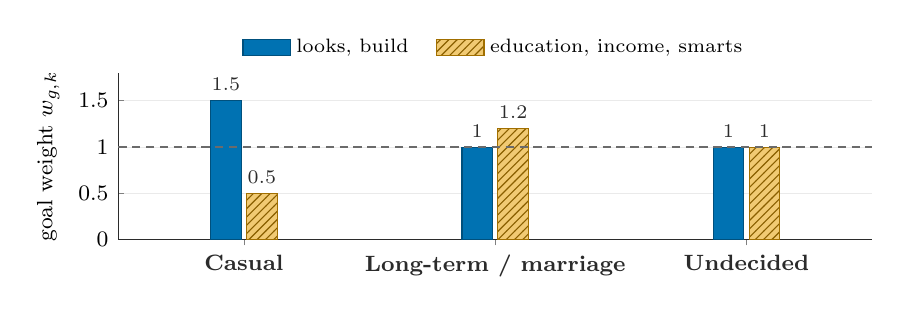
\begin{tikzpicture}
\begin{axis}[
  width=0.92\columnwidth, height=3.7cm,
  ybar, bar width=11pt, ymin=0, ymax=1.8,
  ytick={0,0.5,1,1.5}, ylabel={goal weight $w_{g,k}$},
  ylabel style={font=\footnotesize}, yticklabel style={font=\footnotesize},
  symbolic x coords={Casual,Long-term / marriage,Undecided},
  xtick=data, xticklabel style={font=\footnotesize\bfseries, text=hgink},
  enlarge x limits=0.25,
  nodes near coords, nodes near coords style={font=\scriptsize\bfseries, text=hgink},
  every node near coord/.append style={/pgf/number format/.cd, fixed, precision=1},
  legend style={font=\scriptsize, at={(0.5,1.03)}, anchor=south, draw=none, legend columns=2,
    /tikz/every even column/.append style={column sep=8pt}}, area legend,
  axis lines*=left, axis line style={hgink}, ymajorgrids, grid style={hgink!10},
  major tick length=2pt,
]
\addplot[draw=hgblue!70!black, fill=hgblue] coordinates {(Casual,1.5) (Long-term / marriage,1.0) (Undecided,1.0)};
\addplot[draw=hgorange!70!black, fill=hgorange!55, postaction={pattern=north east lines, pattern color=hgorange!60!black}]
  coordinates {(Casual,0.5) (Long-term / marriage,1.2) (Undecided,1.0)};
\legend{{looks, build},{education, income, smarts}}
\draw[densely dashed, hgink!70, thick] ({rel axis cs:0,0} |- {axis cs:Casual,1}) -- ({rel axis cs:1,0} |- {axis cs:Casual,1});
\end{axis}
\end{tikzpicture}

\caption{Goal weights $w_{g,k}$ of the Hypergamy Meter, exactly as in \texttt{goal\_weight} in \texttt{app/src/model.rs}. \emph{Illustrative}: the values are hand-picked. Only their direction follows the short- versus long-term findings \cite{kenrick1990,likenrick2006}. Age, height, size, red flags and the goal term itself always have weight 1.}
\label{fig:goal}
\end{figure}

\begin{table}[t]
\centering
\caption{Hypergamy Meter contributions in points (hand-picked, not estimated). Ranges show the lowest and highest value per input.}
\label{tab:weights}
\footnotesize
\begin{tabular}{@{}>{\raggedright\arraybackslash}p{1.5cm}>{\raggedright\arraybackslash}p{3.2cm}>{\raggedright\arraybackslash}p{3.2cm}@{}}
\toprule
\textbf{Input} & \textbf{Woman} & \textbf{Man}\\
\midrule
Age & $+12$ at 25--29; $-22$ at 50+ & $+10$ at 30--34; $-10$ at 50+\\
Education$^{a,b}$ & $+4$ Bachelor's; $-8$ PhD & $-6$ high school; $+6$ Master's or PhD\\
Income band$^{b}$ & $-2$ low; $+3$ high & $-10$ low; $+10$ high\\
Height & $-1$ to $+1$ & $-6$ under 170\,cm; $+7$ at 190+\\
Looks$^{c}$ & $-8$ below average; $+11$ head-turner & $-7$ below average; $+10$ head-turner\\
Build$^{c}$ & $-1$ couch potato; $+2$ gym or statue & $-3$ couch potato; $+5$ Greek statue\\
Smarts$^{b}$ & \multicolumn{2}{>{\raggedright\arraybackslash}p{6.2cm}@{}}{$0$ average, $+4$ smart, $+6$ very smart, $+3$ galaxy brain}\\
Size & not asked & $-1$ below average to $+1$\\
Red flags$^{d}$ & \multicolumn{2}{>{\raggedright\arraybackslash}p{6.2cm}@{}}{per flag (0 to 3): $+3$ casual, at most $+8$; $-5$ long-term, at most $-15$; $-8$ marriage, at most $-24$; $0$ undecided; same for everyone}\\
Goal & \multicolumn{2}{l}{$-2$ undecided to $+3$ casual, same for everyone}\\
\midrule
\multicolumn{3}{@{}p{8.3cm}@{}}{\scriptsize Base 60; total clamped to $[0,100]$; height and size are optional; non-binary users get the midpoint, and the man's size row. $^{a}$Multiplied by a region factor: 0.6 Northern Europe, 0.9 North America, 1.0 Latin America, 1.1 Southern Europe, 1.3 Turkey/Middle East, 1.5 East Asia. $^{b}$Multiplied by 0.5 for a casual goal and 1.2 for long-term or marriage. $^{c}$Multiplied by 1.5 for a casual goal. $^{d}$Set by the goal already, so no goal weight applies.}\\
\bottomrule
\end{tabular}
\end{table}

\section{Limitations}
This is a narrative review, not a systematic one, and it leans on Western, mostly US and European, data; work on South and East Asia is thin here apart from Japan \cite{raymo2005}. Several numbers come from abstracts or secondary summaries rather than full texts: the meta-analytic correlations \cite{eastwick2014} (from an author copy), the Tinder match rates \cite{tyson2016}, the OkCupid figures \cite{rudder2009} (an archived company blog) and the gender-equality results of \cite{zentner2012} (from a press release). Beyond status, \cite{stulp2013paid,sorokowski2008,gignac2018,taylor2005} and parts of \cite{mautz2013} are read from secondary summaries, and \cite{curington2021} from its publisher's description. For personality and paternity, \cite{paulhus2002,jonason2015birds,holtzman2010,paulhus1998,jonason2010poach,brewer2015,burger1999,urbaniak2003,mcdaniel2005,marcinkowska2015} are read from secondary summaries, \cite{qureshi2016,lyons2016faces} from metadata or titles only, \cite{aitken2013} from a search summary of its abstract, the sample sizes of \cite{haslam2015} and of the street study in \cite{dufner2013} from press summaries, Baumeister's 80/40 \cite{baumeister2010} from quotations and the 30\% of \cite{anderson2006} from a press release. The Dark Triad data are mostly cross-sectional self-reports. The French legal texts are cited as law, and the French rate is an inference from neighbouring countries. The breadwinner replication \cite{rosenberg2024} is a working paper, and \cite{xia2014} is a preprint. Most evidence beyond status comes from students rating photos, figures or questionnaires, not from real partner choice. Dating-site studies use self-selected users, and fake-profile experiments test first impressions only. Income is measured after marriage, which itself changes earnings. Evidence on same-sex couples is thin \cite{bailey1994,lippa2007,schwartz2009samesex}. Fig.~\ref{fig:reversal} is a schematic, and the app's weights are invented.

\section{Conclusion}
Is hypergamy real? Partly, and it depends which one you mean. Women's stated preference for earning prospects is real, cross-cultural and small per trait. Women still tend to partner with men who earn more and are a few years older. Educational hypergamy was real and has mostly reversed, and supply explains the reversal without any change in what people want. The claims that power the online version (status is all that matters, only women aim up, most women share the top fifth of men) are not supported. Beyond status, the sexes differ most in what they say they want from a long-term partner and least for a casual one. Height, build, penis size and intelligence count in ratings, mostly by small amounts. ``Bad boys'' do get more partners and win first meetings, mostly through looks and boldness, and narcissistic women do too. No study finds them preferred for the long term. Measured misattributed paternity is about 1 to 2\%, not 10 to 30\%. Fewer men than women did pass on their genes, with a female to male effective-size ratio of about 2:1 over the long run and up to 17:1 in the mid-Holocene, and a few founding lines such as N1c spread widely. Why is debated, and none of it describes who fathers children today. The most viral dating-app numbers are blog-grade, and the racial patterns on apps are discrimination, not a measure of anyone's worth. The strongest pattern in the data is the least dramatic one: people mostly pair with people like themselves. If the Hypergamy Meter ever tells you your life is over, believe the bottom caption.

\bibliographystyle{IEEEtran}
\bibliography{bstcontrol,bibliography}

\end{document}
